\documentclass[twocolumn]{article} % Or your preferred document class and options
% !TEX root = main.tex

\usepackage{preamble} % Load your custom preamble


\begin{document}

\coverpage

\begin{abstract}
    abc
\end{abstract}


\section{Introduction}

Quantum-inspired algorithms are classical routines that use mathematical structures and physical intuitions from quantum mechanics — such as superposition-style probability amplitudes, interference or quantum state discrimination — yet run entirely on conventional hardware.  These algorithms have multiple applications, including machine learning, where they promise faster convergence or reduced dimensional dependence compared with traditional methods.

Some machine-learning algorithms are based on dsitance.  Here, the decision rule depends on the similarity between a query sample and a set of prototypes, typically evaluated through dot products or full matrix-vector multiplications.  Although straightforward in software, these operations become a computational bottleneck for high-dimensional data streams or large reference libraries.  There have been optical implementation of classification algorithms (\cite{Psaltis1984}, \cite{Neifeld1993}). Optical information processing offers a compelling alternative: coherent light fields can perform correlations at the speed of propagation, exploiting spatial parallelism while consuming only milliwatts of power.



Among the various optical architectures, the \emph{Joint Transform Correlator} (JTC) stands out for its simplicity and adaptability.  Unlike classical VanderLugt systems, the JTC does not require a pre-fabricated filter; instead, the reference and query patterns are placed side by side in the input plane.  A single Fourier transform—implemented with a lens—produces an output intensity whose off-axis terms encode the cross-correlation between the two patterns.  When feature vectors are encoded as two-dimensional phase distributions, the correlation peak height provides a direct measure of their similarity, which can be mapped to a distance-based decision rule.

In this work we propose an optical implementation of the Quantum-Inspired Nearest Mean Classifier that uses a single SLM and a 1-f lens system.  We begin by reviewing the theoretical connection between optical correlation and amplitude-based similarity measures. We then describe our experimental set-up, which integrates a reflective, phase only, spatial light modulator and a CMOS camera to implement a proof-of-concept optical classifier (Section~\ref{sec:setup}).  Finally, we benchmark the model with the MNIST dataset and compare its performance with a purely electronic implementation, highlighting the trade-offs in speed, energy, and classification accuracy (Section~\ref{sec:results}).


\section{Theory}

\subsection{Machine learning and supervised classification}
\subsection{Quantum-inspired classification}
\subsection{Joint Transform Correlator}

\section{Results}

\begin{table}[htbp]
  \centering
  \caption{Classification accuracy (mean $\pm$ std.)}
  \label{tab:cls-results}
  \begin{tabular}{@{}lll c@{}}
    \toprule
    Classifier & Distance metric & Encoding & Accuracy (\%)\\ 
    \midrule
    RBF-C & Euclidean & - & - \\
    RBF-C & JTC & - & - \\[2pt]
    CNM-C & Euclidean & — & $80.38 \pm 0.38$ \\ 
    CNM-C & JTC & — & $72.42 \pm 0.55$ \\[2pt]
    QNM-C & Trace     & Standard     & \textbf{$85.84 \pm 0.38$} \\ 
    QNM-C & Fidelity  & Standard     & $78.77 \pm 0.34$ \\[2pt]
    QNM-C & Trace     & Informative  & $81.26 \pm 0.37$ \\ 
    QNM-C & Fidelity  & Informative  & \textbf{$82.39 \pm 0.40$} \\ 
    \bottomrule
  \end{tabular}
\end{table}




\section{Data Encoding}
\subsection{Gram Matrix Encoding}

We consider a column vector $u$ representing an image sample. To embed this into a higher-order representation, we construct the normalized outer product:
\[
\rho = \frac{uu^T}{\text{Tr}(uu^T)}
\]
This yields a density-like matrix $\rho$ with trace 1, encoding pairwise correlations between pixels. Such an encoding is inspired by quantum mechanical density operators and preserves structural information in the image.

\begin{figure}[h!]
    \centering
    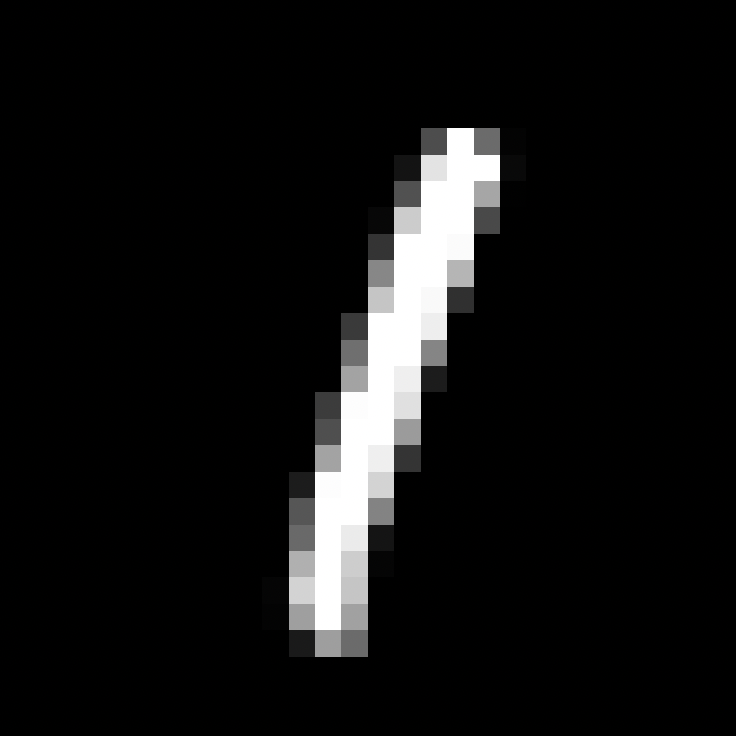
\includegraphics[width=0.6\linewidth]{figures/nmist_1_data.png}
    \caption{Example MNIST image (digit 1)}
    \label{fig:dataset_one}
\end{figure}

\begin{figure}[h!]
    \centering
    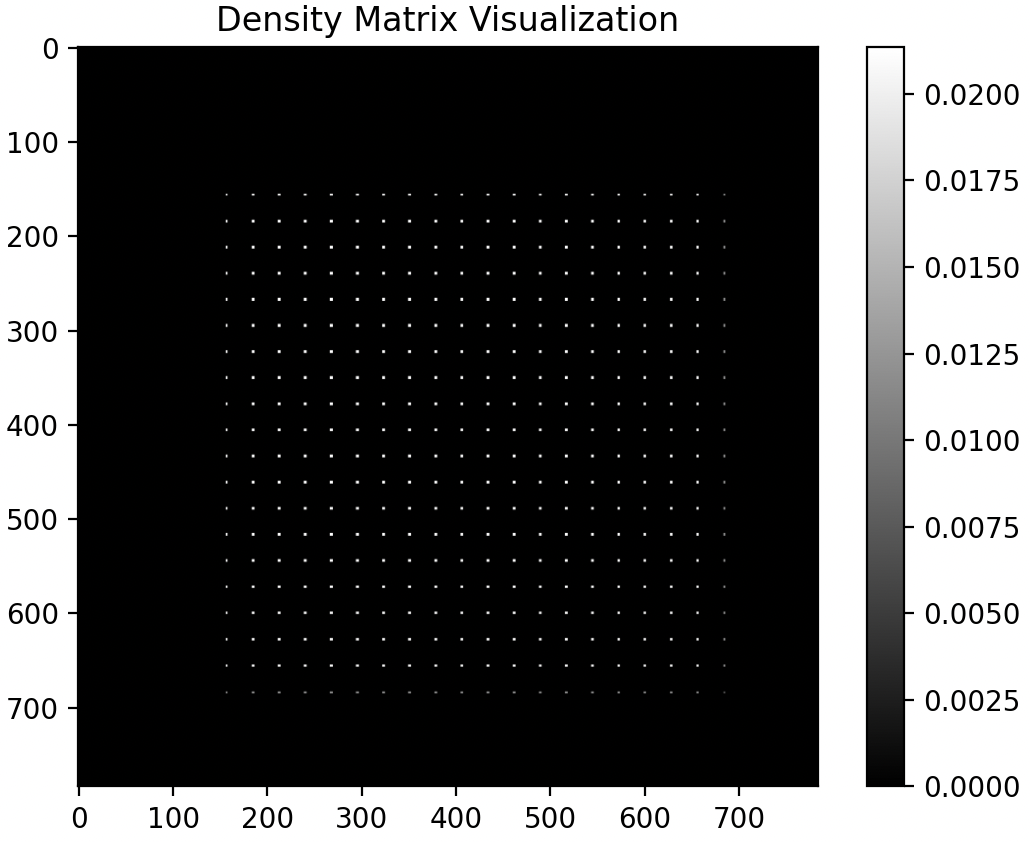
\includegraphics[width=0.6\linewidth]{figures/density_matrix_nmist_one.png}
    \caption{Gram matrix encoding $\rho$ of the digit 1 image}
    \label{fig:density_matrix}
\end{figure}

\section{Radial Basis Function Network}

RBF networks model the hypothesis function $h(x)$ using a radial function centered around key points (called \emph{centers}). Each center influences the prediction based on its proximity to the input $x$. The standard form is:
\[
h(x) = \sum_{n=1}^N w_n\exp\left(-\gamma\| x - x_n \|^2\right)
\]
where $\gamma$ determines the width of the radial functions, and $w_n$ are the learned weights.

\subsection{Exact Interpolation}
Given training data $D = \{(x_1, y_1), \dots, (x_N, y_N)\}$, we can formulate the interpolation condition:
\[
\sum_{m=1}^N w_m\exp\left(-\gamma\| x_n - x_m \|^2\right) = y_n, \quad \forall n
\]
In matrix notation:
\[
\Phi \mathbf{w} = \mathbf{y}, \quad \text{where } \Phi_{n,m} = \exp\left(-\gamma\|x_n - x_m\|^2\right)
\]
If $\Phi$ is invertible, we can directly solve:
\[
\mathbf{w} = \Phi^{-1} \mathbf{y}
\]
This yields an exact interpolating function.

\subsection{Classification}
For classification, we apply a decision rule such as:
\[
h(x) = \operatorname{sign}\left(\sum_{n=1}^N w_n\exp(-\gamma\|x - x_n\|^2)\right)
\]
In multi-class settings, this can be extended to a softmax output over class scores.

\subsection{Training with Least Squares}
Instead of enforcing exact interpolation, we may use a least squares approach to minimize:
\[
E = \sum_{n=1}^N (h(x_n) - y_n)^2
\]
This leads to the ridge-regularized solution:
\[
\mathbf{w} = (\Phi^T\Phi + \lambda I)^{-1}\Phi^T \mathbf{y}
\]
where $\lambda$ is a regularization parameter.

\section{Choosing RBF Centers}
Using every data point as a center is computationally expensive. Instead, we reduce the number of centers to $K \ll N$ by clustering the dataset using \textbf{K-Means}:

We define:
\[
J = \sum_{k=1}^K \sum_{x_n \in S_k} \| x_n - \mu_k \|^2
\]
and use Lloyd's algorithm to iteratively minimize $J$:
\begin{align*}
\mu_k &= \frac{1}{|S_k|}\sum_{x_n \in S_k} x_n \\
S_k &= \{ x_n : \|x_n - \mu_k\| \leq \|x_n - \mu_j\|,\ \forall j \neq k \}
\end{align*}

Repeat these steps until convergence. Since the process is sensitive to initialization, we typically run K-Means multiple times and choose the best clustering.

\begin{figure}[h!]
    \centering
    % Consider plotting a 3D Gaussian RBF here with Gnuplot
    \begin{gnuplot}[scale=0.6, terminal=pdf]
set title "3D Gaussian Function"
set xlabel "x"
set ylabel "y"
set zlabel "z"
set hidden3d
set view 60, 80
set isosamples 50, 50
set xrange [-5:5]
set yrange [-5:5]

# Parameters for the Gaussian
sigma = 1.0
mu_x = 0.0
mu_y = 0.0

# 2D Gaussian Function
gaussian(x, y) = exp(-((x - mu_x)**2 + (y - mu_y)**2) / (2 * sigma**2))

splot gaussian(x, y) with lines palette
\end{gnuplot}
    \caption{Example of a Gaussian RBF centered at $\mu$}
    \label{fig:gaussian_rbf}
\end{figure} 

\section{Implementation Notes}
The RBF network was implemented in Python using NumPy and scikit-learn. To avoid memory issues, we:
\begin{itemize}
    \item Use MiniBatchKMeans to find centers efficiently.
    \item Use perceptron-based or regularized least squares learning.
    \item Avoid computing large $\Phi^T\Phi$ matrices when possible.
\end{itemize}

\section{Optical Im}

\section{Conclusion}
RBF networks provide an elegant and powerful framework for classification. Through Gaussian kernel construction and data-driven center selection, they can adapt to local structures in the data. When combined with efficient encodings such as Gram matrices and practical training algorithms, they scale to real-world tasks like digit recognition.

\bibliography{references}{}
\bibliographystyle{plain}

\end{document}
